\subsection{Przegląd architektur zamkniętych pętli sterowania ENI}\hypertarget{sec:25}{}

\subsubsection{Wstęp}

Niniejsze pętle zostały przedstawione w kontekście późniejszej analizy, która będzie miała na celu wywiedzenie wymagań na platformę. Opis powstał na podstawie \cite{etsieni2024}, który analizuje architektury zamkniętych pętli sterowania w celu wykorzystania ich w swojej modularnej architekturze. //TODO to jest jednak już ta analiza

\subsubsection{Typy pętli sterowania}

Większość architektur pętli sterowania dla systemów kognitywnych i adaptywnych używa mechanizmów:
\begin{itemize}
    \item sprzężenia zwrotnego (ang. \textit{ang. feedback}) - mechanizm, w którym system reaguje na swoje wyjście i dostowosuje swoje działanie na podstawie wyników,
    \item sprzężenia wyprzedzającego (ang. \textit{ang. feedforward}) - mechanizm, w którym system przewiduje przyszłe zmiany i podejmuje działania, zanim błąd faktycznie się pojawi.
\end{itemize}

Te sygnały odgrywają kluczową rolę w stabilizowaniu systemu, ale też jego umiejętności empirycznego uczenia się. Pętlę, która wykorzystuje mechanizm feedbacku nazywamy \textbf{zamkniętą}.

\textbf{Hierarchiczna} koordynacja (organizacja) pętli przypomina drzewo. Organizacja ta pozwala, aby różne decyzje podejmowane były przez rożne węzły drzewa. W ogólności, istnieje zestaw nadrzędnych (ang. \textit{supervisory}) pętli, które alokują zadania do pętli podwładnych (ang. \textit{subordinary}). Każda podrzędna pętla wykonuje swoje zadania i zwraca rezultaty do swojej pętli nadrzędnej. 

Zaawansowane zastosowania pozwalają jednej grupie dedykowanych pętli przejąć kontrolę nad hierarchią w zależności od celów i zmian w środowisku. 


\begin{figure}[!h]
    \centering 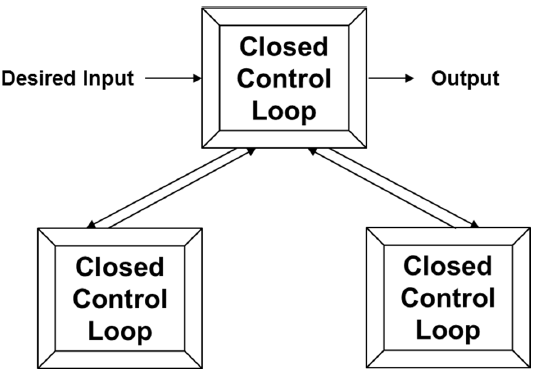
\includegraphics[width=1\linewidth]{25-hierachical.png}
    \caption{Hierarchiczna organizacja zamkniętych pętli sterowania}\label{fig:25-hierachical}
\end{figure}

Pętla \textbf{rozproszona} składa się z komponentów działających w różnych lokalizacjach, które komunikują się ze sobą poprzez mechanizmy przesyłania wiadomości. 

\textbf{Adaptacyjność} pętli to dostosowywanie jej parametrów sterowania w czasie rzeczywistym albo na podstawie modelu, który definiuje pożądany efekt, albo używając analizy statystycznej do budowania modelu na podstawie mierzonych danych.

\textbf{Federacją} nazywamy grupę pół autonomicznych pętli sterowania, które używają formalnych kontraktów, aby regulować ich wzajemną interakcję i zachowania. Kontrakty obejmują zasady przyjmowania nowych członków federacji, regulacje dotyczące widoczności i rodzaju informacji jakie mogę być udostępnianie innym członkom federacji. Każda pętla federacji operuje na swoich lokalnych danych. Następnie decyzje podjęte przez każdą z nich są agregowane i publikowane jako wspólna decyzja federacji.

\textbf{Kognitywną} pętla sterowania nazywamy taką, która z pośród dostępnych jej danych jest w stanie wyrozumować nowe dane, informację i finalnie wiedzę, która pomoże jej osiągać cele zarządzania.

\subsubsection{OODA}
Architektura pętli OODA \cite{boyd1995} jest widoczna na Rysunku \ref{fig:25-ooda}.

Widoczne jest iż, każdy element posiada komunikację na trzech płaszczyznach:
\begin{itemize}
    \item Otrzymanie danych od poprzedniego elementu lub środowiska zewnętrznego
    \item Przekazanie feedbacku do elementu "Observe" (za wyjątkiem "Orient")
    \item Przekazanie danych do następnego elementu lub środowiska zewnętrznego
\end{itemize}

Dodatkowo element "Orient" może przekazywać swoje dane do elementów "Observe" oraz "Act". Ze środowiskiem zewnętrznym komunikować mogą się jedynie elementy "Observe" oraz "Act", z czego każdy w innym kierunku. Mimo, iż pętla wydaje się być sekwencyjna, jest to złudzenie. Każdy element działa nieustannie a pobudzanie go do działania działa na zasadzie otrzymania danych.

//TODO Teraz to zdanie należy przerobić na wymaganie w sekcji badawczej

\begin{figure}[!h]
    \centering 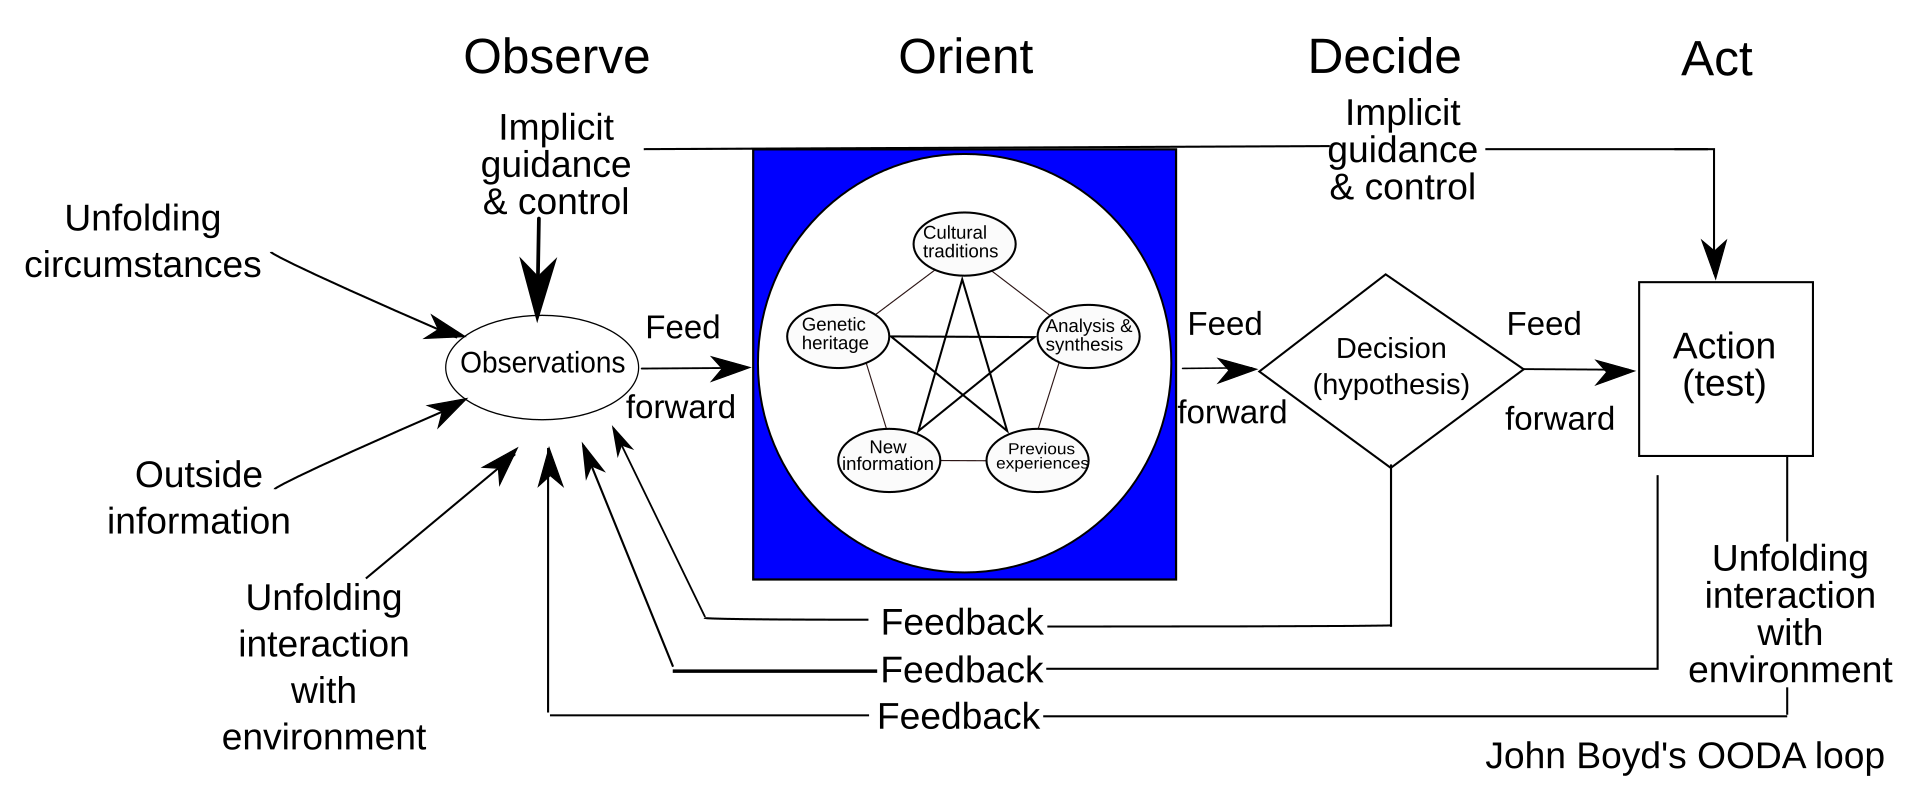
\includegraphics[width=1\linewidth]{25-ooda.png}
    \caption{Architektura pętli OODA}\label{fig:25-ooda}
\end{figure}

\subsubsection{MAPE-K}
Architektura pętli MAPE-K \cite{kephart2003} jest widoczna na Rysunku \ref{fig:25-mapek}.

Jest to pętla sekwencyjna, każdy element komunikuje się jedynie na dwóch płaszczyznach otrzymując dane od poprzedniego (lub środowiska zewnętrznego w przypadku "Monitor") i przekazując dane następnemu elementowi (lub do środowiska zewnętrznego w przypadku "Execute"). Dodatkowo każdy element podłączony jest do "Knowledge", które stanowi wspólne repozytorium wiedzy. Generowanie oraz konsumpcja wiedzy stanowi oddzielną komunikację i nie wpisuje się w \hyperlink{def:workflow}{\textit{workflow pętli}}. 

\begin{figure}[!h]
    \centering 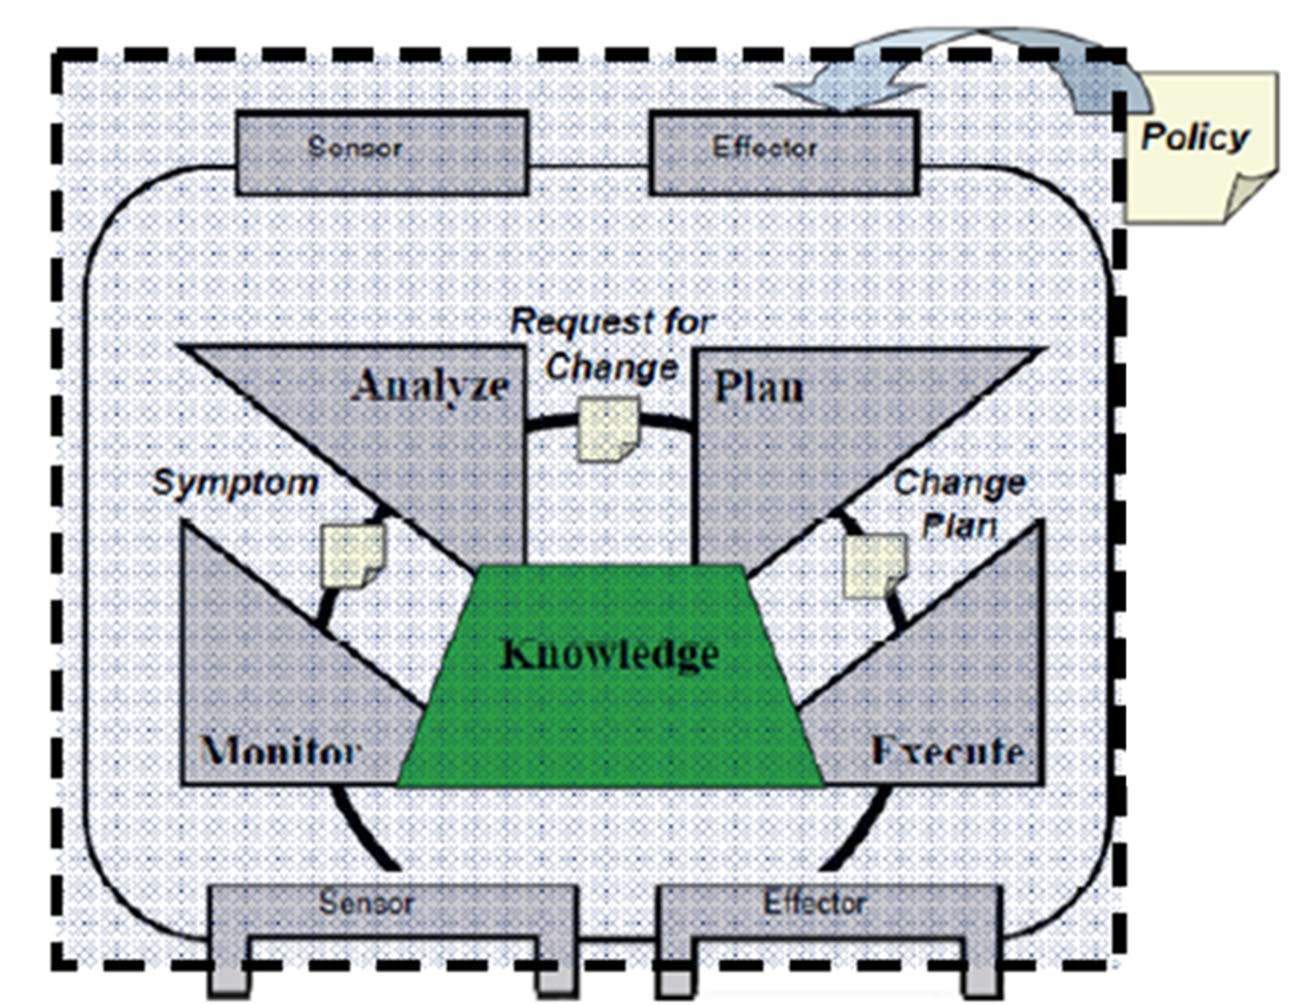
\includegraphics[width=1\linewidth]{25-mapek.png}
    \caption{Architektura pętli MAPE-K}\label{fig:25-mapek}
\end{figure}

\subsubsection{Focale}
Architektura pętli Focale \cite{strassner2007} jest widoczna na Rysunku \ref{fig:25-focale}. Workflow pętli jest sekwencyjne, ale z drugiej strony za pomocą wspólnej szyny danych każdy element może komunikować się z każdym. Ważnym atrybutem szyny jest to, że natywnie wspiera ona model informacji DEN-ng \cite{strassner2003} oraz ontologii DENON-ng \cite{strassner2007}. Widzimy tu też podłączony do każdego elementu "Autonomic Manager", koncept z \cite{kephart2003}. Focale w każdej iteracji może przyjąć inny przebieg. Mówimy tu o pętli utrzymaniowej, czyli przebiegu, który zachodzi w przypadku gdy system zarządzany nie wymaga żadnych akcji naprawczych lub optymalizacyjnych. Kiedy stan aktualny nie zgadza się ze stanem pożądanym, pętla przybiera przebieg rekonfiguracyjny.

\begin{figure}[!h]
    \centering 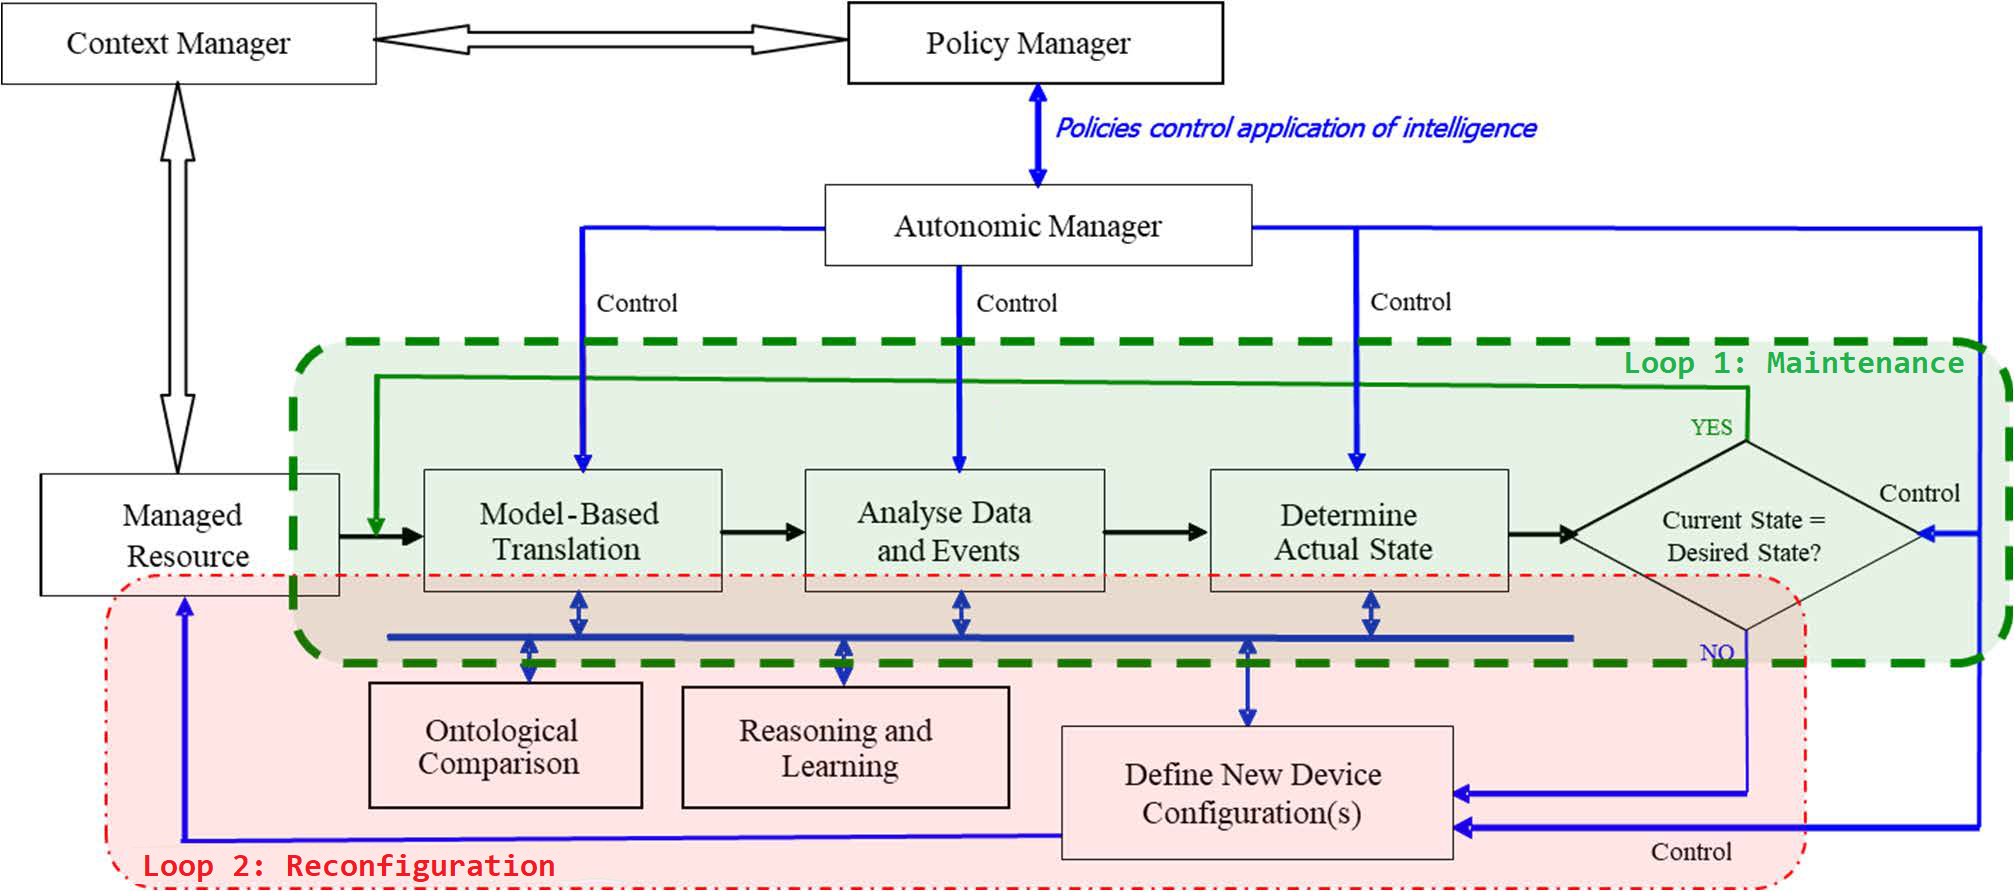
\includegraphics[width=1\linewidth]{25-focale.png}
    \caption{Architektura pętli Focale}\label{fig:25-focale}
\end{figure}

\subsubsection{GANA}
Architektura GANA (Generic Autonomic Network Architecture) \cite{etsigana2018} jest widoczna na Rysunku \ref{fig:25-gana}. Nie jest to konkretna pętla a raczej zestaw wielu hierarchicznych pętli sterowania. Pętle najniższego poziomu implementują tzw. szybkie pętle sterowania, które korzystają z kognitywności w najmniejszym stopniu (lub wcale). Idąc w górę hierarchi, stopień wykorzystania podejścia kognitywnego rośnie, a co za tym idzie pętle stają się coraz wolniejsze. 

\begin{figure}[!h]
    \centering 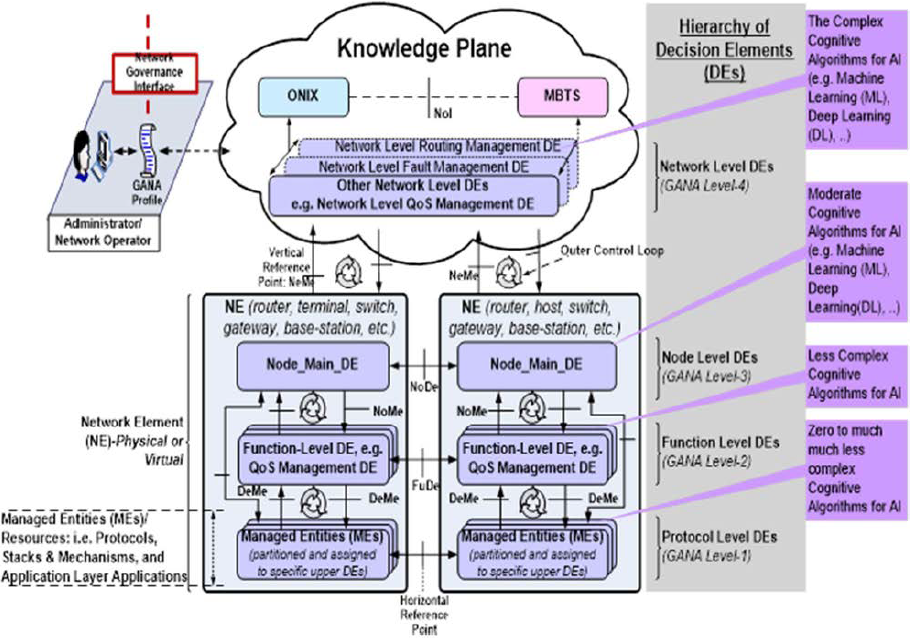
\includegraphics[width=1\linewidth]{25-gana.png}
    \caption{Architektura pętli GANA}\label{fig:25-gana}
\end{figure}

\subsubsection{COMPA}
Architektura pętli COMPA (Control, Orchestration, Management, Policies, Analytics) \cite{doyle2014} jest widoczna na Rysunku \ref{fig:25-compa}. Samo workflow pętli nie przynosi nic nowego ponadto co w poprzednich pętlach. Wartym uwagi jest jednak to, że systemem zarządzanym (tu "automation target") jednej pętli COMPA, może być inna instancja pętli COMPA, co wprowadza rekurencję. 

\begin{figure}[!h]
    \centering 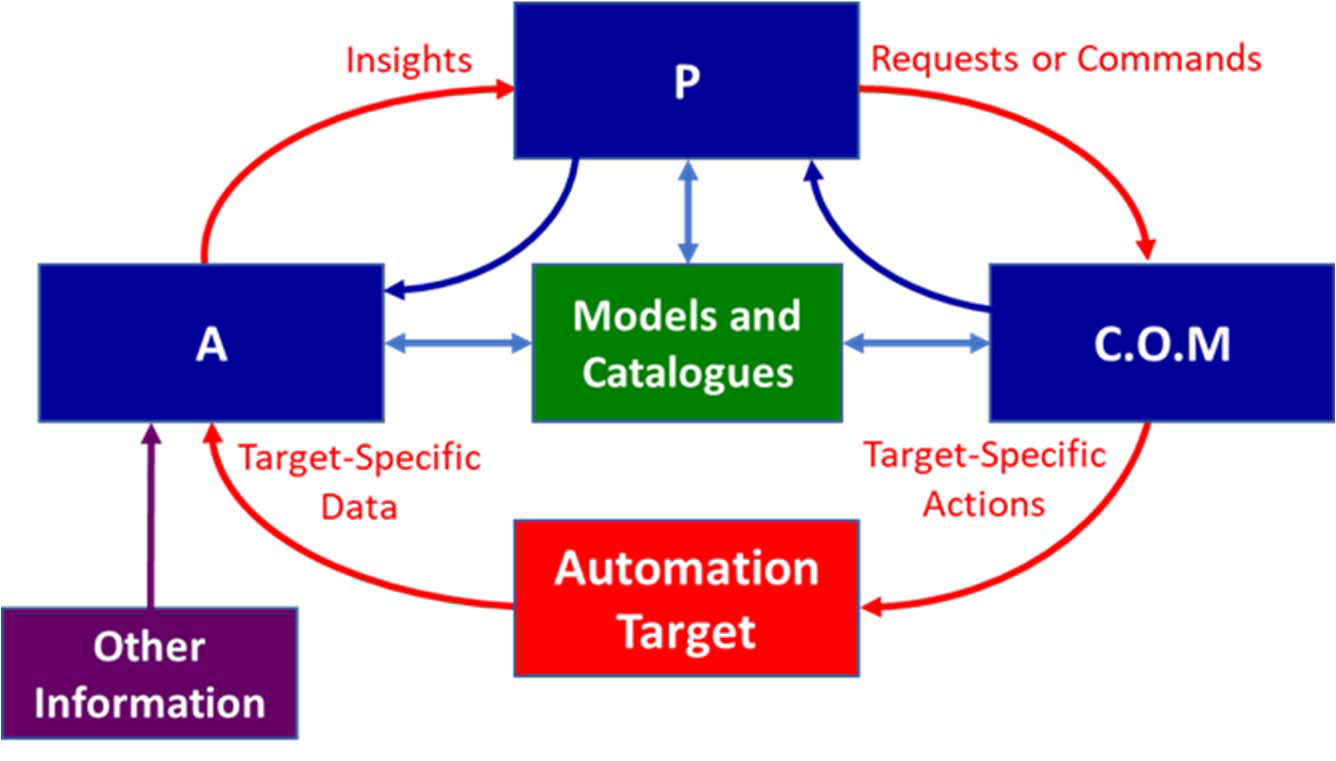
\includegraphics[width=1\linewidth]{25-compa.png}
    \caption{Architektura pętli COMPA}\label{fig:25-compa}
\end{figure}

\subsubsection{Focale v3}
Architektura pętli Focale v3 \cite{strassner2009} jest widoczna na Rysunku \ref{fig:25-focalev3}. Jest to kolejna wersja architektury Focale, która to zamiast używać dwóch alternatywnych pętli proponuje dwie nieustannie działające pętle. Jedna zewnętrzna, używana do rekoncylacji systemu zarządzanego na większą skale w ramach reagowanie na zmiany kontekstu środowiska. Druga wewnętrzna, do rekoncylacji w ramach jednego określone kontekstu (sytuacji) np. w jednej iteracji. Obie mają 3 alternatywne przebiegi inspirowane \cite{minsky1986}. Przebieg reaktywny używany jest w wypadku gdy zmiany kontekstu już kiedyś się wydarzyły i były przeanalizowane. Przebieg obradujący (ang. \textit{deliberative}) jest wykorzystywany gdy zmiana kontekstu jest zmiana, ale jej detale nie są jeszcze do końca zrozumiane, aby podjąć natychmiastową akcję. Przebieg refleksyjna ma miejsce, gdy zachodzą zupełnie nowe zmiany kontekstu i system musi się "nauczyć z nimi radzić. W kontekście komunikacji elementów wersja ta nie wnosi nic poza to co pętla FOCALE.

\begin{figure}[!h]
    \centering 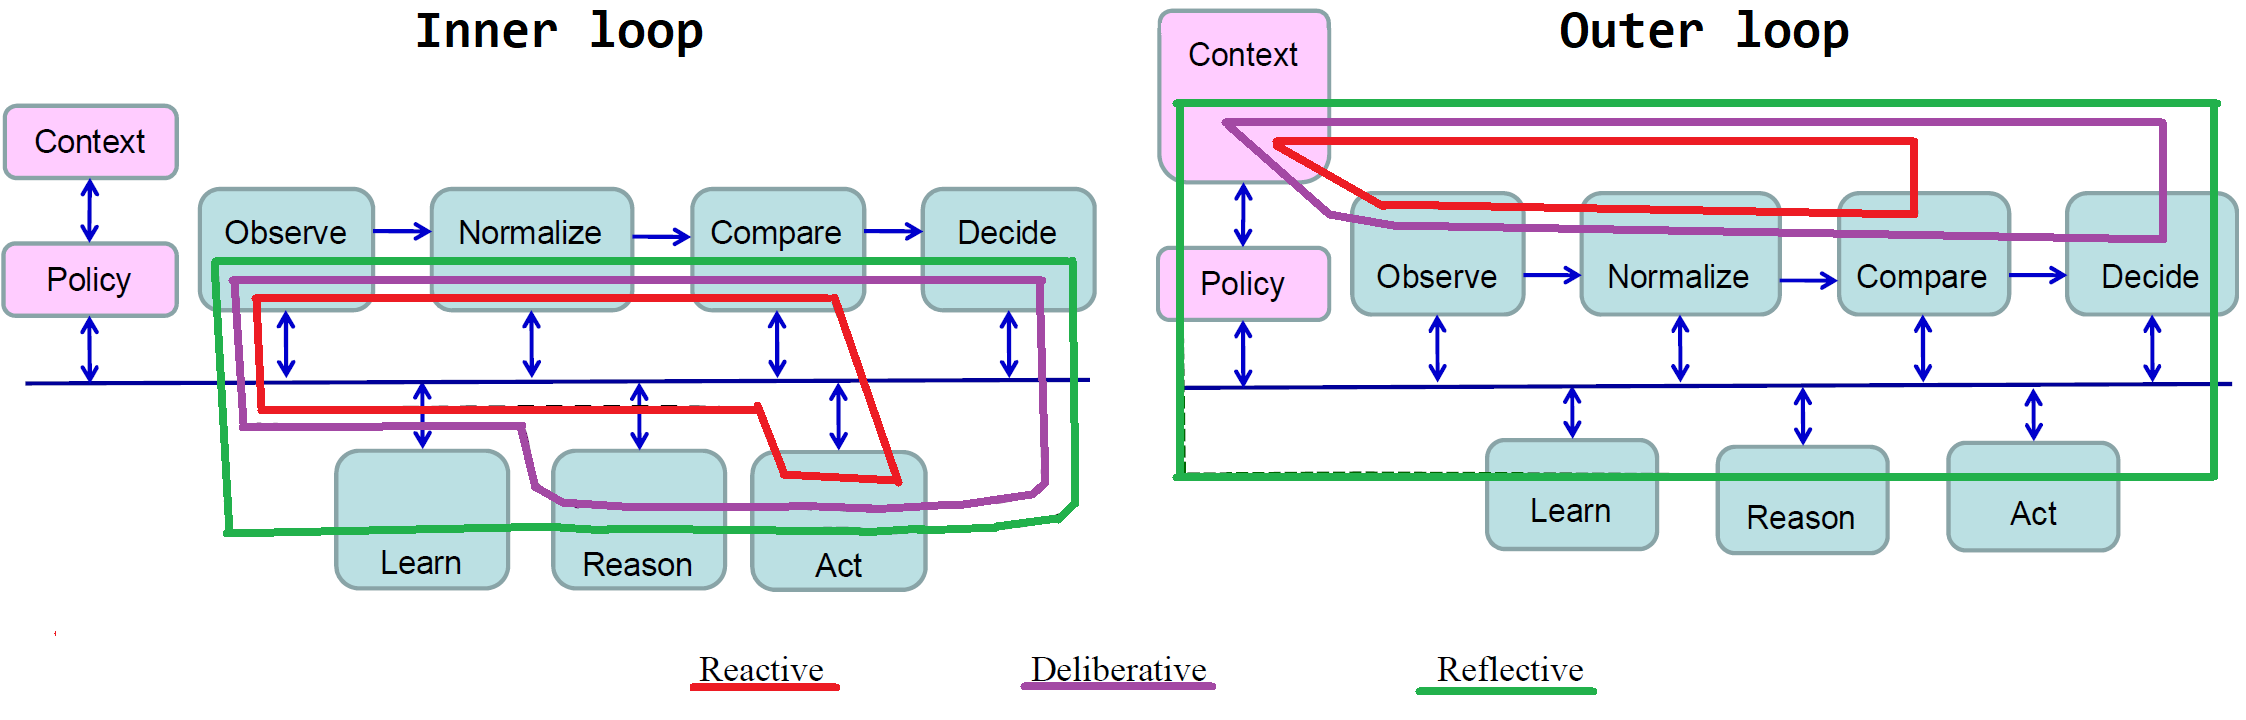
\includegraphics[width=1\linewidth]{25-focalev3.png}
    \caption{Architektura pętli Focale v3}\label{fig:25-focalev3}
\end{figure}
